\documentclass[english,a4paper,12pt,oneside]{article}


%\includeonly{lab4}

%Drafting options
%uncomment for double spacing
%\doublespacing

% \usepackage{acronym}
\usepackage{times}
\usepackage{setspace} 
\usepackage{amsmath}    % need for subequations
\usepackage{graphicx}   % need for figures
%\usepackage{picture}
% \usepackage{wrapfig}
\usepackage{graphics}
 \graphicspath{{./}{../data/}}
 \usepackage{epstopdf}
\usepackage{color}
\usepackage{listings}
\lstset{basicstyle=\ttfamily\footnotesize,
	breaklines=true,
%    basicstyle=\ttfamily,
    keywordstyle=\color{blue}\ttfamily,
    stringstyle=\color{red}\ttfamily,
    commentstyle=\color{magenta}\ttfamily,
%    morecomment=[l][\color{magenta}]{\#}
}
\usepackage{verbatim}   % useful for program listings
\usepackage{color}      % use if color is used in text
\usepackage{subfigure}  % use for side-by-side figures
\usepackage{varioref}
\usepackage{anysize}
\usepackage{natbib}
\usepackage{fancyhdr}
% \usepackage{units}
\usepackage{longtable}
%\usepackage{bbding}
%\usepackage{aeguill}
\usepackage[hyphens]{url}
\usepackage{hyperref}

\setlength{\parskip}{8pt plus 2pt minus 2pt}
\setlength{\parindent}{0pt}

\marginsize{2cm}{2cm}{2cm}{2cm}
\fancypagestyle{plain}{%
  \fancyhf{}%
  \renewcommand{\headrulewidth}{0pt}%
  \renewcommand{\footrulewidth}{0pt}%
}

\pagestyle{fancy}
%\renewcommand{\sectionmark}[1]{\markright{\thesection.\ #1}}

\renewcommand{\sectionmark}[1]{\markright{#1}{}}
\renewcommand{\subsectionmark}[1]{\markright{#1}{}}
\renewcommand{\subsubsectionmark}[1]{\markright{#1}{}}

%\renewcommand{\quote}[1]{\textit{\begin{quote}#1\end{quote}}}
\newcommand{\bold}[1]{\emph{\textbf{#1}}}

\newcommand{\varentry}[1]{{\guillemotleft}\emph{#1}{\guillemotright}}
\newcommand{\code}[1]{{\tt #1}}

\headheight 10mm


\rhead{Semester 2}
\chead{Lab 9}
\lhead{ICP3038 --- Computer Vision}
\rfoot{}
\cfoot{- \thepage  \,\,-}
\lfoot{}

\renewcommand{\headrulewidth}{0.4pt}
\renewcommand{\footrulewidth}{0.4pt} 



%%%%%%%%%%%%%%%%%%%%%%%%%%%%%%%%%%%%%%%%%%%%%%%%%%%%%%%%%%%%%%%%%%%%%%%%%%%%%%%%
\begin{document}


%%%%%%%%%%%%%%%%%%%%%%%%%%%%%%%%%%%%%%%%%%%%%%%%%%%%%%%%%%%%%%%%%%%%%%%%%%%%%%%%
\section*{Laboratory 9: Playing a video from a file or the webcam}


The aims of today's lab are:
\begin{itemize}
	\item Playing a video from a file;
	\item Playing a video from a webcam;
	\item Process the input frames;
	\item Display two images side by side in the same window;
	\item Saving a video stream in a file (CAREFUL, they can become big).
\end{itemize}
The point is to use a video stream (from a file or a camera) and do some image processing on the incoming frames. You will then adapt this lab to create your own motion detection algorithm. 

To achieve these goals, we will create several programs:
\begin{enumerate}
	\item \verb+videoFromFile.cxx+: A simple program using OpenCV to display a video and perform some image processing tasks (this file is provided);
	\item \verb+videoFromWebCam.cxx+: A similar program where the video stream comes from a webcam (there is webcam on most laptops and on the PCs in the lab) (this file is not provided).
\end{enumerate}
You are provided with the skeleton of \verb+videoFromFile.cxx+. 
% Add it to the \verb+CMakeLists.txt+ file from last week.

Everything we did last week is relevant for today's session. 
You are also expected to have completed Lab~7 already as we need to convert an image from greyscale (binary in fact) to RGB. 

\begin{tabular}{cc}

\includegraphics[width=0.15\linewidth]{UK_traffic_sign_562}&
\begin{minipage}[b]{0.8\textwidth}
\textbf{Note for Mac users:}\\
I had problem OpenCV from Homebrew using my Macbook Pro.
I had to re-install it using the command line as follows:\\
\end{minipage}
\end{tabular}
\begin{description}
%\item[OpenCV 2.x:]\verb+brew install opencv --with-ffmpeg --with-libdc1394+
\item[OpenCV 3.x:]\verb+brew install opencv3 --with-ffmpeg --with-libdc1394 --with-qt5+
\item[OpenCV 4.x:]\verb+brew install opencv4 --with-ffmpeg --with-libdc1394 --with-qt5+
\end{description}


%%%%%%%%%%%%%%%%%%%%%%%%%%%%%%%%%%%%%%%%%%%%%%%%%%%%%%%%%%%%%%%%%%%%%%%%%%%%%%%%
\newpage
\section{Video from a file}
 
We will write the code in \verb+videoFromFile.cxx+.
The program takes three arguments from the command line:
\begin{itemize}
  \item The input video file;
  \item A scaling factor to resize the input data (use `1' for no scaling);
  \item The output video file (optional).
\end{itemize}

Test videos can be found at:
\begin{itemize}
\item \url{http://www.mysticfractal.com/video/avi1.html}
\item \url{http://techslides.com/sample-files-for-development}
\item \url{http://www.technical-recipes.com/2011/displaying-avi-video-using-opencv/}
\item \url{http://www.engr.colostate.edu/me/facil/dynamics/avis.htm}
\end{itemize}

We will display a window with two images, the input and the output, side by side (see Fig.~\ref{fig:screenshot}).
 \begin{figure}[htbp]
  \centering
  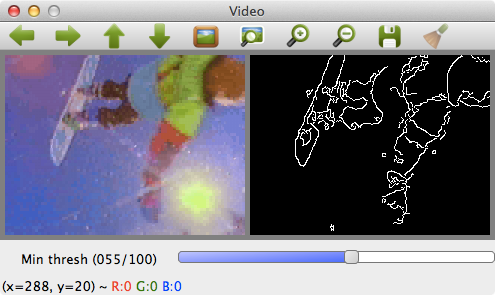
\includegraphics[width=0.7\linewidth]{screenshot1}
  \caption{\label{fig:screenshot}Screenshot.}
 \end{figure}

 \newpage
\subsection{Global Variables}

First of all, we need some global variables:

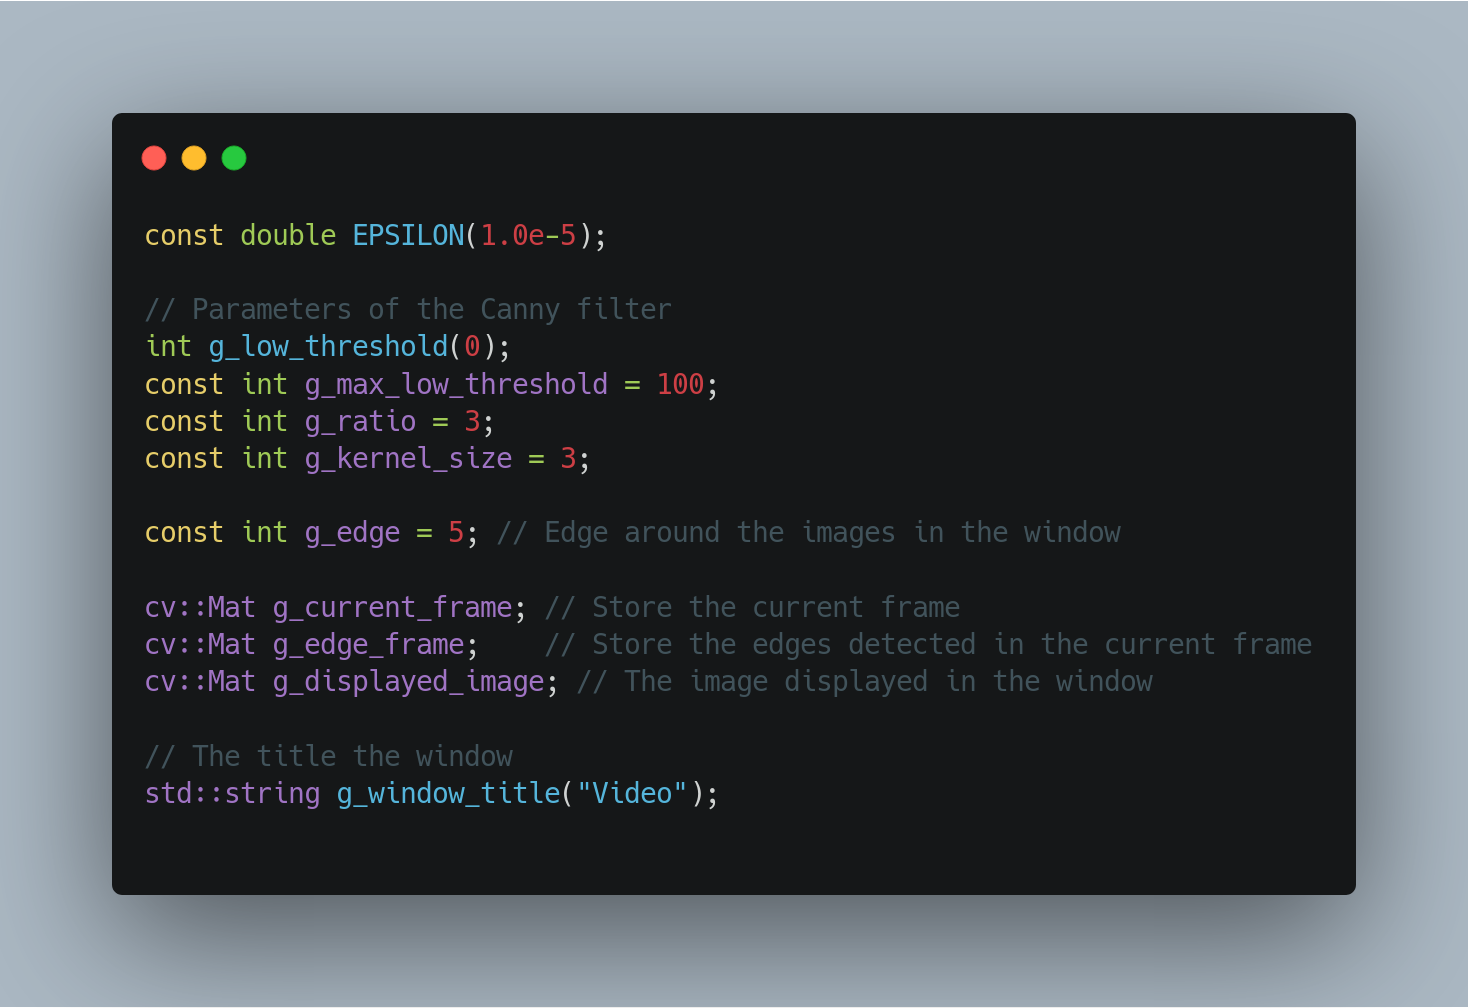
\includegraphics[width=\linewidth]{/home/fpvidal/Downloads/carbon}
% \begin{lstlisting}[language=c++]
% const double EPSILON(1.0e-5);
% 
% // Parameters of the Canny filter
% int g_low_threshold(0);
% const int g_max_low_threshold = 100;
% const int g_ratio = 3;
% const int g_kernel_size = 3;
% 
% const int g_edge = 5; // Edge around the images in the window
% 
% cv::Mat g_current_frame; // Store the current frame
% cv::Mat g_edge_frame;    // Store the edges detected in the current frame
% cv::Mat g_displayed_image; // The image displayed in the window
% 
% // The title the window
% std::string g_window_title("Video");
% \end{lstlisting}


 \newpage
\subsection{Opening the video stream}
\label{sec:param}

The class corresponding to video streams, either from files or cameras, is \verb+cv::VideoCapture+. 
To opening a stream, use the constructor:

% \begin{lstlisting}[language=c++]
% // Open the video file
% cv::VideoCapture video_capture(input_file_name);
% \end{lstlisting}
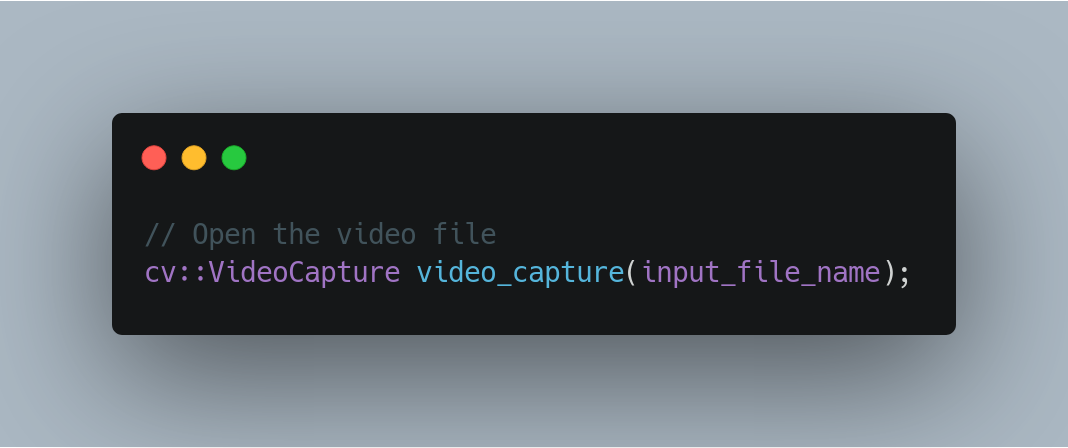
\includegraphics[width=\linewidth]{/home/fpvidal/Downloads/carbon(1)}

Always check if an error occurred, and if it did, throw an error:

% \begin{lstlisting}[language=c++]
% // The image has not been loaded
% if (!video_capture.isOpened())
% {
%     // Create an error message
%     std::string error_message;
%     error_message  = "Could not open or find the video \"";
%     error_message += input_file_name;
%     error_message += "\".";
% 
%     // Throw an error
%     throw error_message;
% }
% \end{lstlisting}
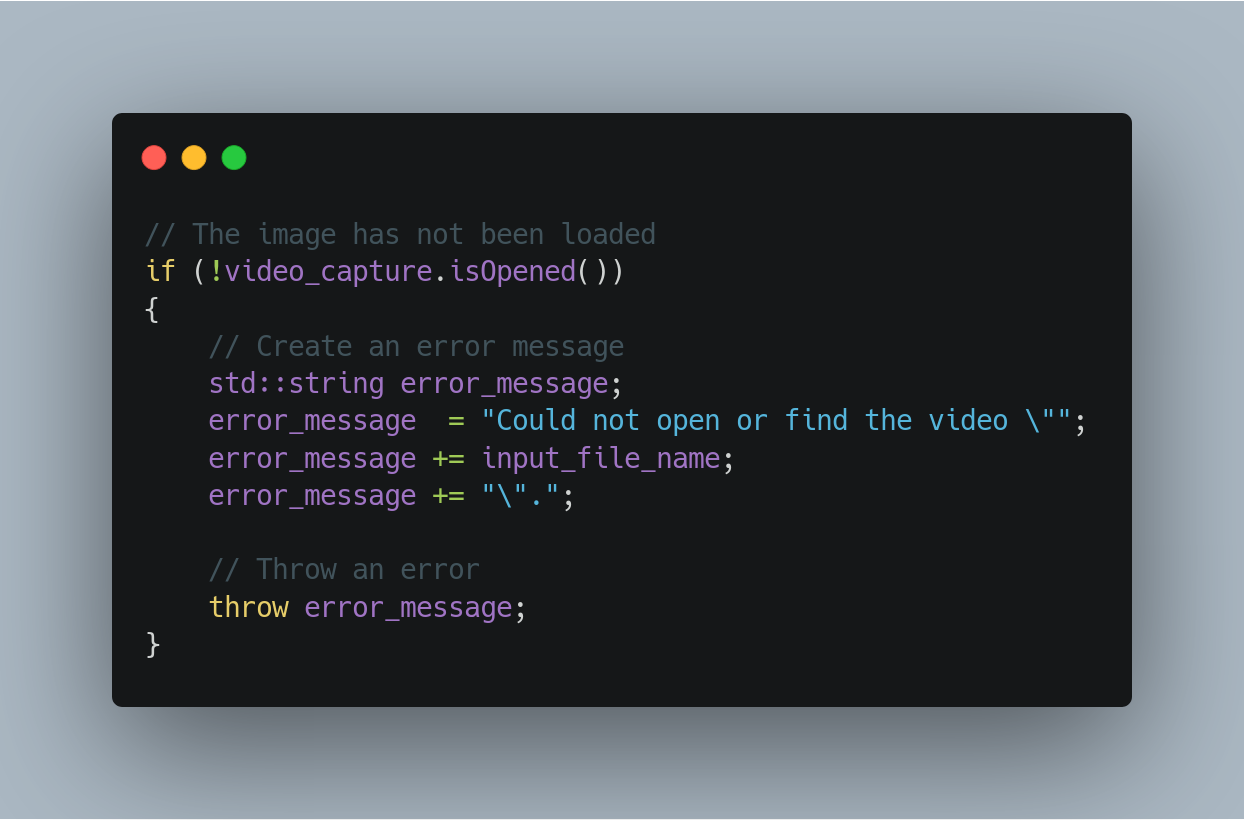
\includegraphics[width=\linewidth]{/home/fpvidal/Downloads/carbon(2)}

Now we need to read the framerate and the image size:

% \begin{lstlisting}[language=c++]
% // Read the frame rate of the video (does not always work)
% double fps = video_capture.get(CV_CAP_PROP_FPS);  
% cout << "Frame per seconds: " << fps << endl;
% 
% // Convert in seconds per frame
% double seconds_per_frame(1.0 / fps);
% 
% // Convert in milliseconds
% int milliseconds_per_frame(round(seconds_per_frame * 1000.0));
% 
% // Get the video size
% cv::Size input_video_size(video_capture.get(CV_CAP_PROP_FRAME_WIDTH),
% 		video_capture.get(CV_CAP_PROP_FRAME_HEIGHT));
% \end{lstlisting}
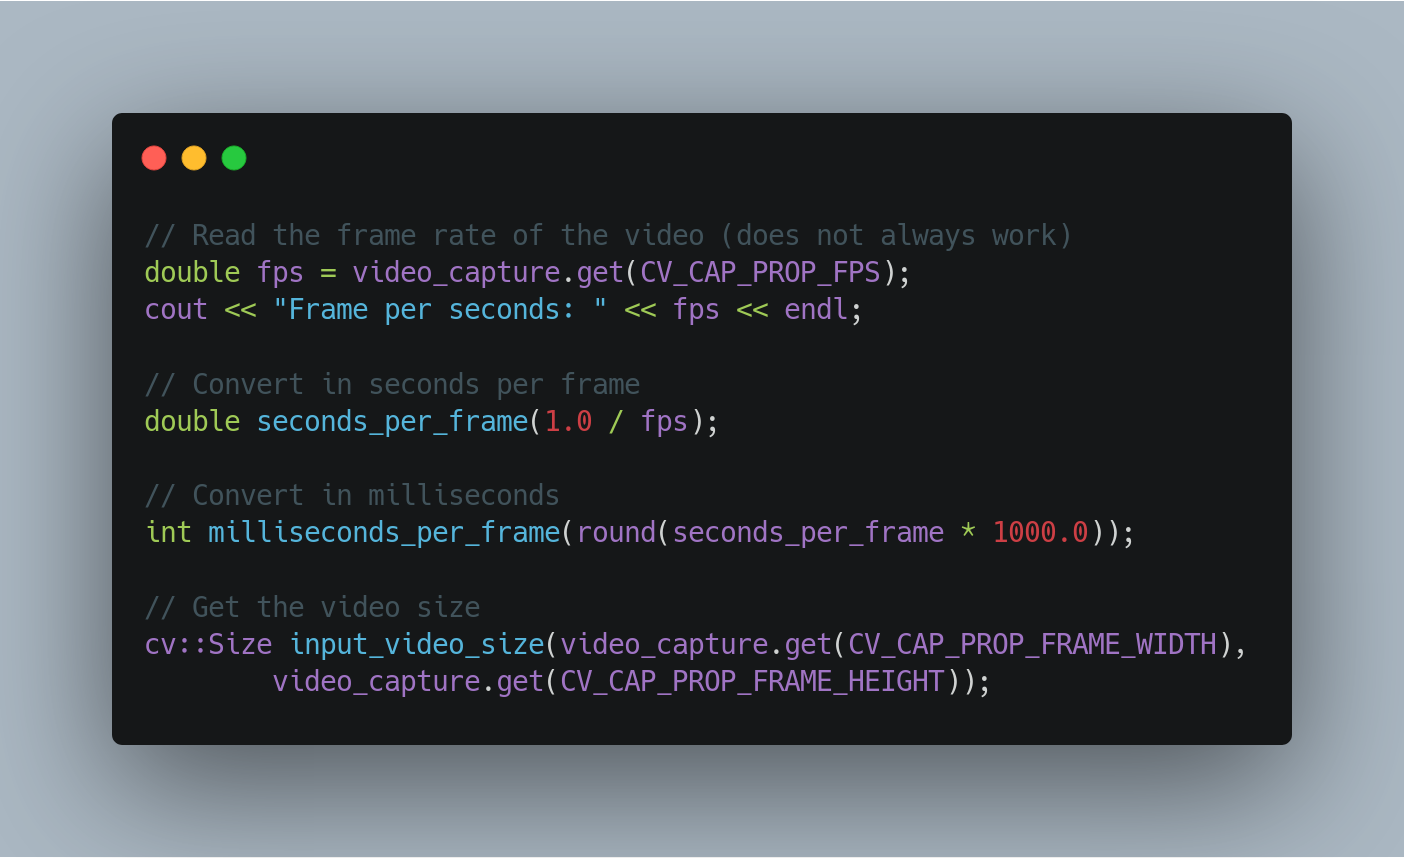
\includegraphics[width=\linewidth]{/home/fpvidal/Downloads/carbon(3)}



We can now compute the image size when the scaling factor is applied and the size of the image that will be displayed in the window:

% \begin{lstlisting}[language=c++]
% // Apply the scaling factor
% cv::Size scaled_video_size(input_video_size.width * scaling_factor,
%         input_video_size.height * scaling_factor);
% 
% // Set the size of the image displayed in the window
% cv::Size target_video_size(g_edge * 3 + 2 * scaled_video_size.width,
%         g_edge * 2 + scaled_video_size.height);
% \end{lstlisting}
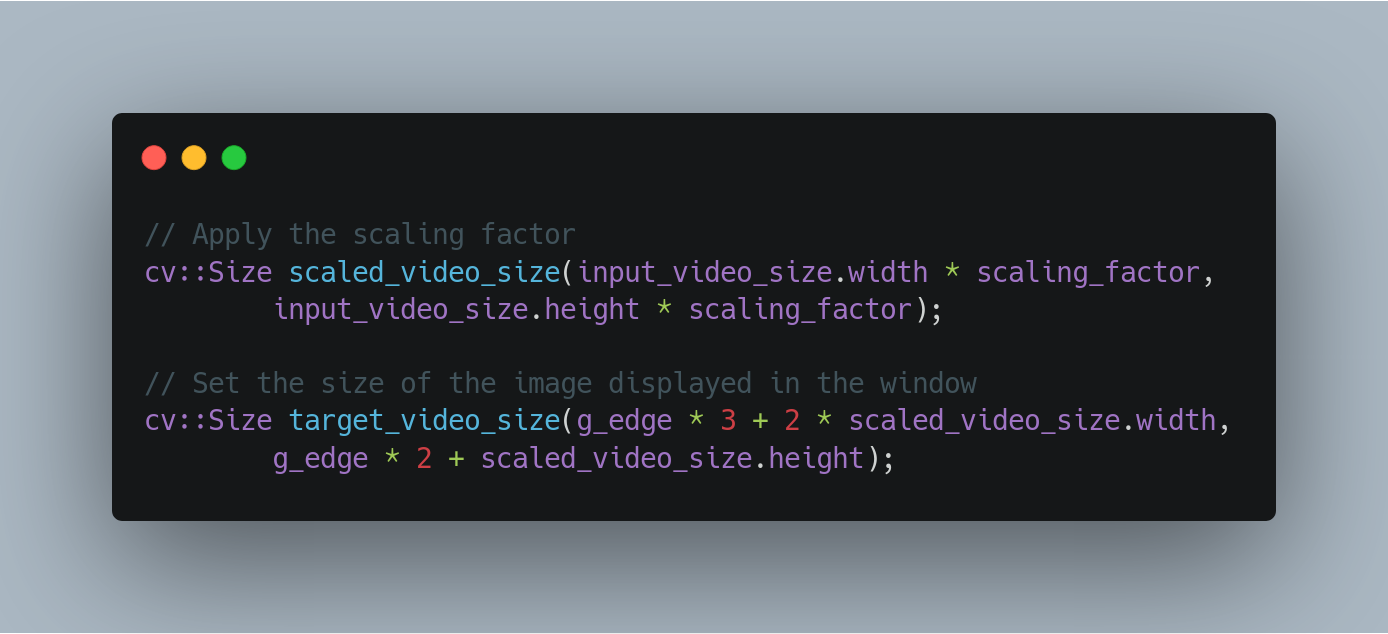
\includegraphics[width=\linewidth]{/home/fpvidal/Downloads/carbon(4)}

We are now ready to create our new RGB image with the default colour [128, 128, 128]:

% \begin{lstlisting}[language=c++]
% // Create the output image
% g_displayed_image = cv::Mat(target_video_size.height,
%         target_video_size.width,
%         CV_8UC3,
%         cv::Scalar(128, 128, 128));
% \end{lstlisting}
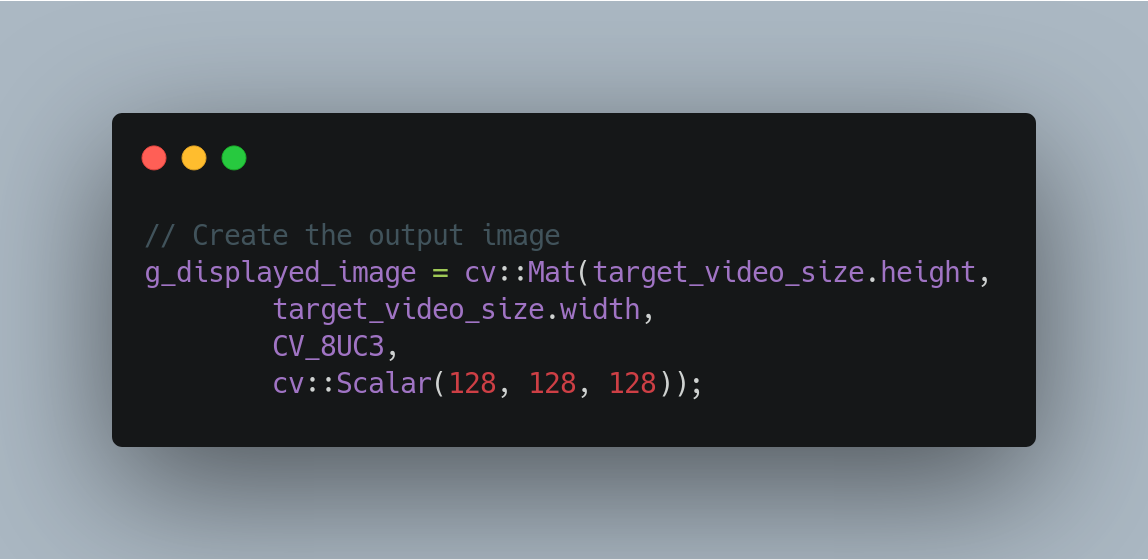
\includegraphics[width=\linewidth]{/home/fpvidal/Downloads/carbon(5)}


\newpage
\subsection{Setting the file writer}
The class needed to write a file is \verb+cv::VideoWriter+. 
You will need to specify a file name and a codec when you open the file. 
To get the codec of the input video stream, use:

% \begin{lstlisting}[language=c++]
% int input_codec = video_capture.get(CV_CAP_PROP_FOURCC);
% \end{lstlisting}
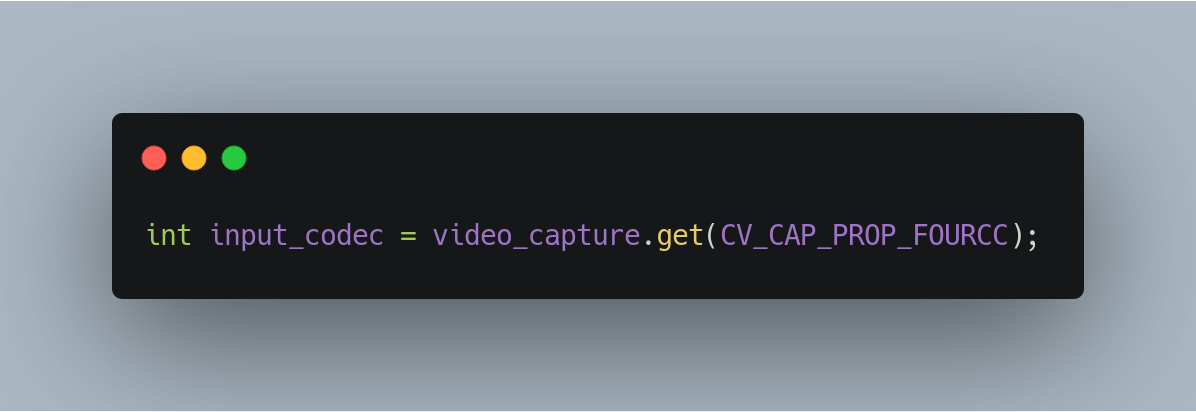
\includegraphics[width=\linewidth]{/home/fpvidal/Downloads/carbon(6)}

To open the file, you need:

% \begin{lstlisting}[language=c++]
% // video_writer.open(output_file_name, input_codec, fps, target_video_size, true);
% \end{lstlisting}
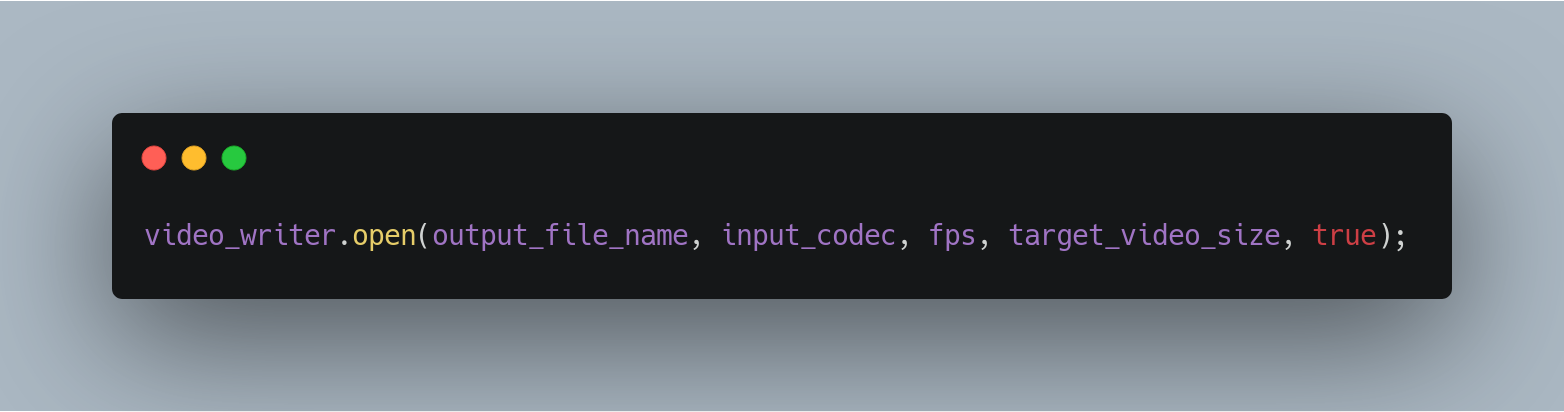
\includegraphics[width=\linewidth]{/home/fpvidal/Downloads/carbon(7)}

You can notice the \verb+fps+ and \verb+target_video_size+ are used here to specify the properties of the video stream. 

Below is the code you can use to open the output file:

% \begin{lstlisting}[language=c++]
% // // Get the codec of the input video
% int input_codec = video_capture.get(CV_CAP_PROP_FOURCC);
% 
% // Open the file writer with the same codec as the input
% video_writer.open(output_file_name, input_codec, fps, target_video_size, true);
% 
% // The file is not open
% if (!video_writer.isOpened())
% {
% 	// Open the file writer with another codec
% 	video_writer.open(output_file_name, CV_FOURCC('M', 'J', 'P', 'G'), fps, target_video_size, true);
% 
% 	// The file is not open
% 	if (!video_writer.isOpened())
% 	{
% 		// Display an error message
% 		std::cerr << "WARNING: Cannot create the output video." << std::endl;
% 	}
% }
% \end{lstlisting}
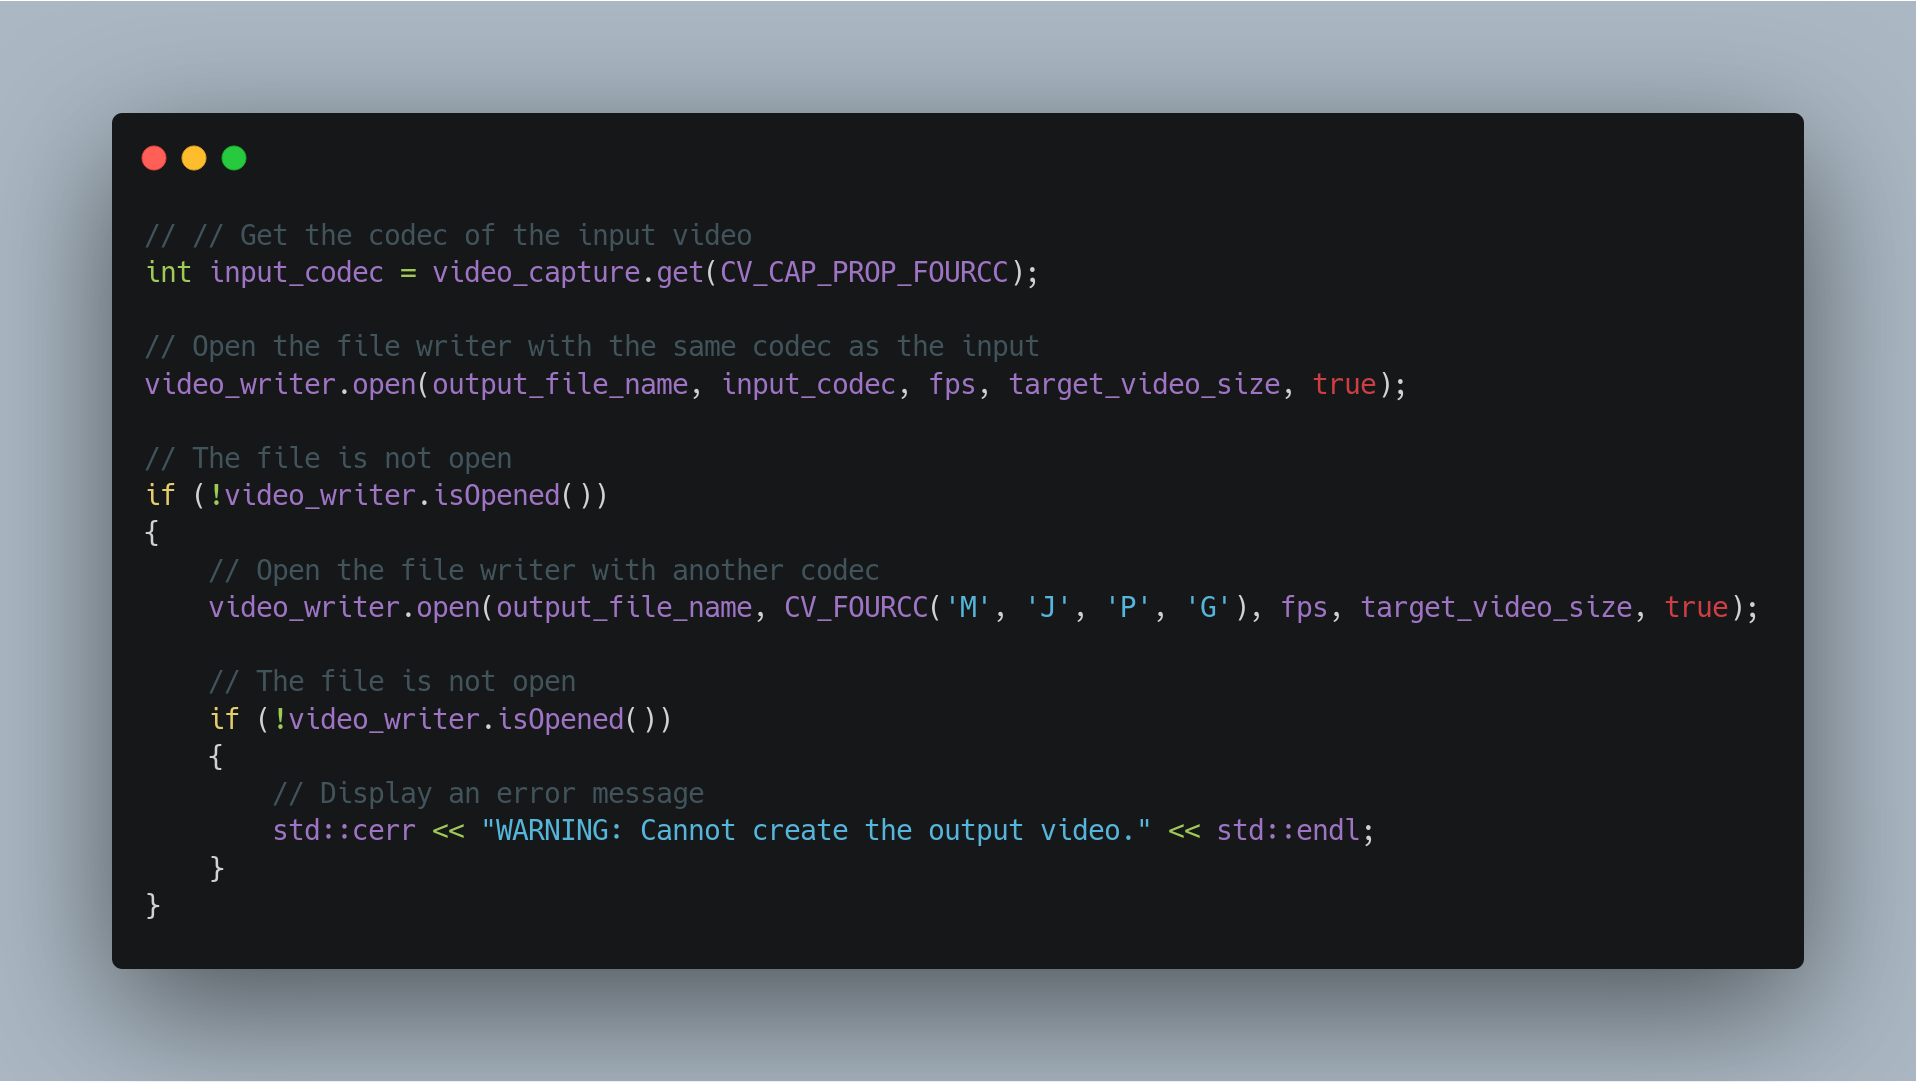
\includegraphics[width=\linewidth]{/home/fpvidal/Downloads/carbon(8)}

First we try to open the file with the same codec as the input file. 
If it does not work, we try a codec that is provided by OpenCV directly. 
Its drawback is that it produces large files as each frame is saved in JPEG. 


\subsection{Create the window and track bar}

We saw last week how to do create a window with a track bar. 
The variable that we want to control is \verb+g_low_threshold+. 
Its upper limit is \verb+g_max_low_threshold+. 
The callback function is \verb+cannyThreshold+.


\newpage
\subsection{Reading a frame}

We read frames in a loop of the form:


% \begin{lstlisting}[language=c++]
% // Last key pressed
% int key;	
% 
% // Input stream status
% bool input_stream_status(true);
% 
% // Event loop
% do
% {
%     // Grab the next frame if possible
%     ...
%         
%     // The image was read from the video stream
%     if (input_stream_status)
%     {
%         // Resize the input if needed
%         if (input_video_size != scaled_video_size)
%         {
%             ...
%         }
%     
%         // Process the image
%         CannyThreshold(0, 0);
%     
%         // The file writer is working
%         if (video_writer.isOpened())
%         {
%             // Add the current frame to the video output
%             ...
%         }
%     
%         // Wait for the key press event or for X ms
%         // (with X equal to 'milliseconds_per_frame')
%         key = cv::waitKey(milliseconds_per_frame);
%     }
% }
% // Stop the loop if 'q' or 'Escape' have been pressed or there is no image left in the video stream
% while (key != 'q' && key != 27 && input_stream_status);
% \end{lstlisting}
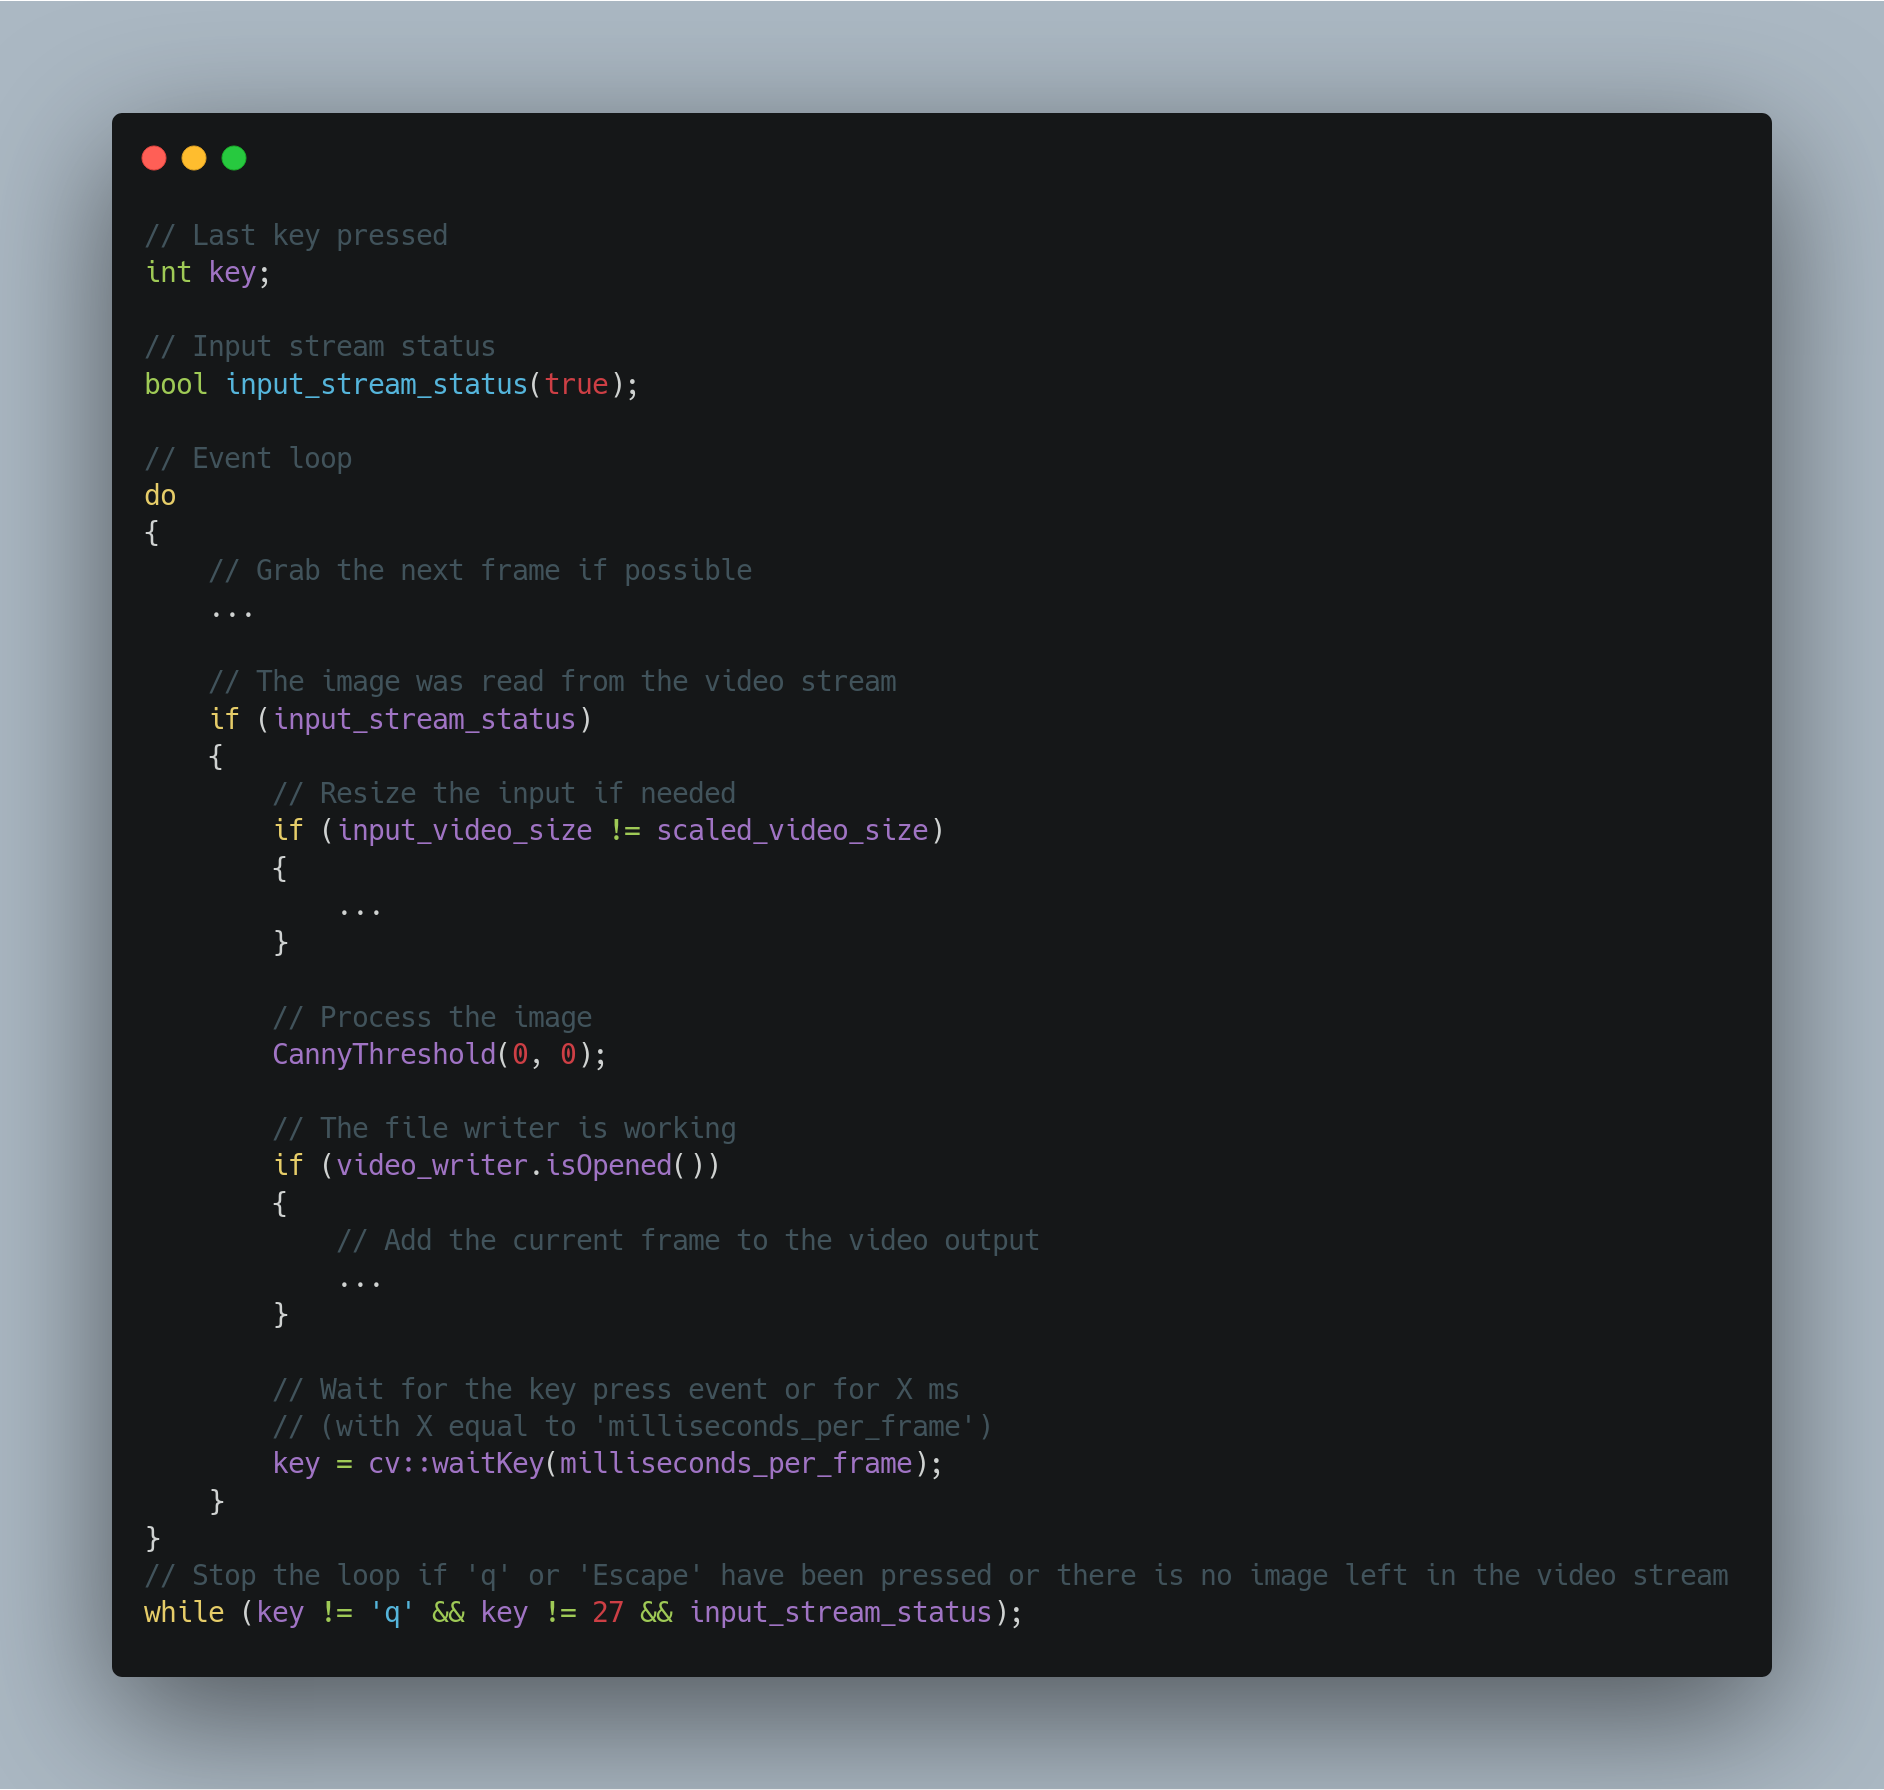
\includegraphics[width=\linewidth]{/home/fpvidal/Downloads/carbon(9)}

We use a \verb+do-while+ loop to make sure that at least one image is processed. 
We start by getting a new frame from the stream and check if an error occurred (e.g.~no more frame to read). 
If the input size has been changed, we rescale the frame.
Then the image processing step is performed in the \verb+CannyThreshold+ callback then the new image is added to the output stream if needed. 
We now wait for the key press event or for $X$ milliseconds with $X=$\verb+milliseconds_per_frame+ (computed in Section~\ref{sec:param}).


To get a frame, we use:

% \begin{lstlisting}[language=c++]
% input_stream_status = video_capture.read(g_current_frame);
% \end{lstlisting}
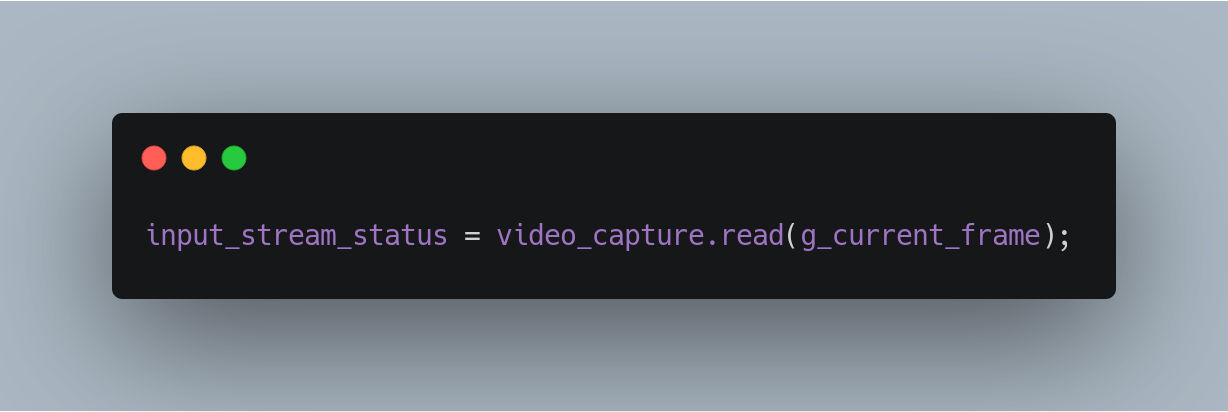
\includegraphics[width=\linewidth]{/home/fpvidal/Downloads/carbon(10)}

It returns a boolean value, which is \verb+true+ if the function call was successful. 
If it returned \verb+false+, then there is no processing to do and the loop can end. 


To resize the frame, use:

% \begin{lstlisting}[language=c++]
% if (input_video_size != scaled_video_size)
% {
%     cv::resize(g_current_frame, g_current_frame, scaled_video_size);
% }
% \end{lstlisting}
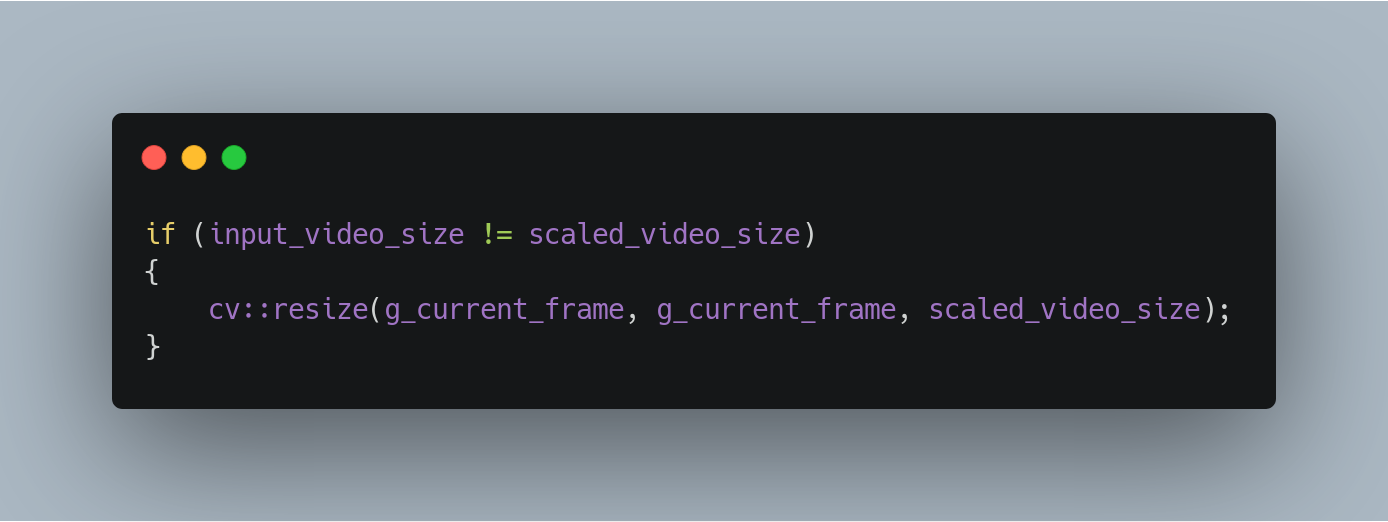
\includegraphics[width=\linewidth]{/home/fpvidal/Downloads/carbon(11)}

To add a frame to the output video stream, use:

% \begin{lstlisting}[language=c++]
% video_writer.write(g_displayed_image);
% \end{lstlisting}
% or
% \begin{lstlisting}[language=c++]
% video_writer << g_displayed_image;
% \end{lstlisting}

\begin{center}
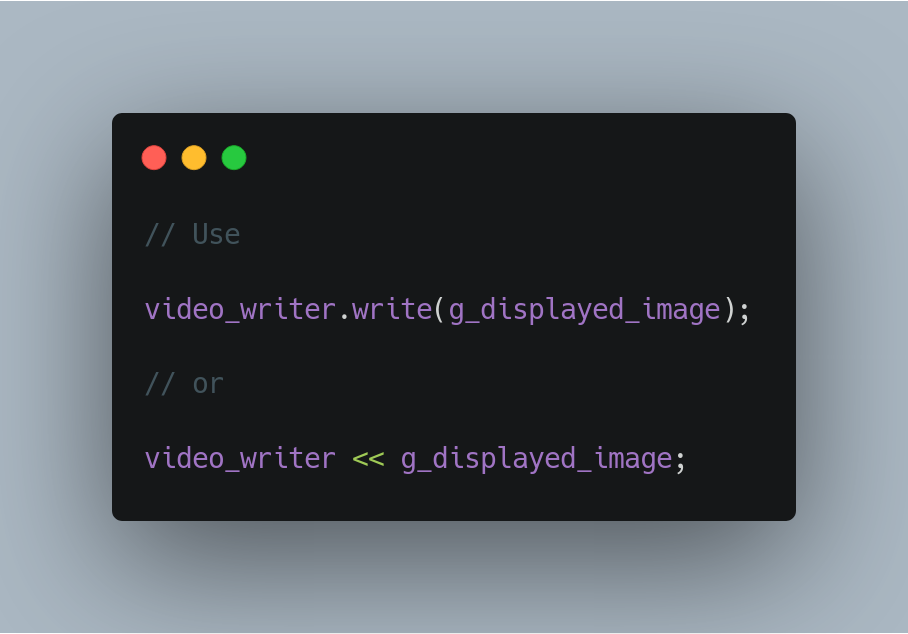
\includegraphics[width=0.6\linewidth]{/home/fpvidal/Downloads/carbon(12)}
\end{center}

%            // Grab the next frame if possible
%            // If an error occured, throw an error
%            if (!video_capture.read(g_current_frame))
%            {
%                // Throw an error
%                throw "Could not read frames from the video.";
%            }
%        
%            // Resize the input if needed
%            if (input_video_size != scaled_video_size)
%            {
%                cv::resize(g_current_frame, g_current_frame, scaled_video_size);
%            }
%




\subsection{Image processing step}

The code is written in the callback function. 
This is why we needed global variables. 

First, reduce the amount of noise with a $3 \times 3$ Gaussian filter (or box filter).

Then copy the input image into a region of interest (ROI) within the image that will be displayed (we called it \verb+g_displayed_image+). 
With the code as follows, we leave an edge of $N$ pixels around the image (with $N=$ \verb+g_edge+):

% \begin{lstlisting}[language=c++]
% cv::Mat targetROI = g_displayed_image(cv::Rect(g_edge, g_edge, g_current_frame.cols, g_current_frame.rows));
% g_current_frame.copyTo(targetROI);
% \end{lstlisting}
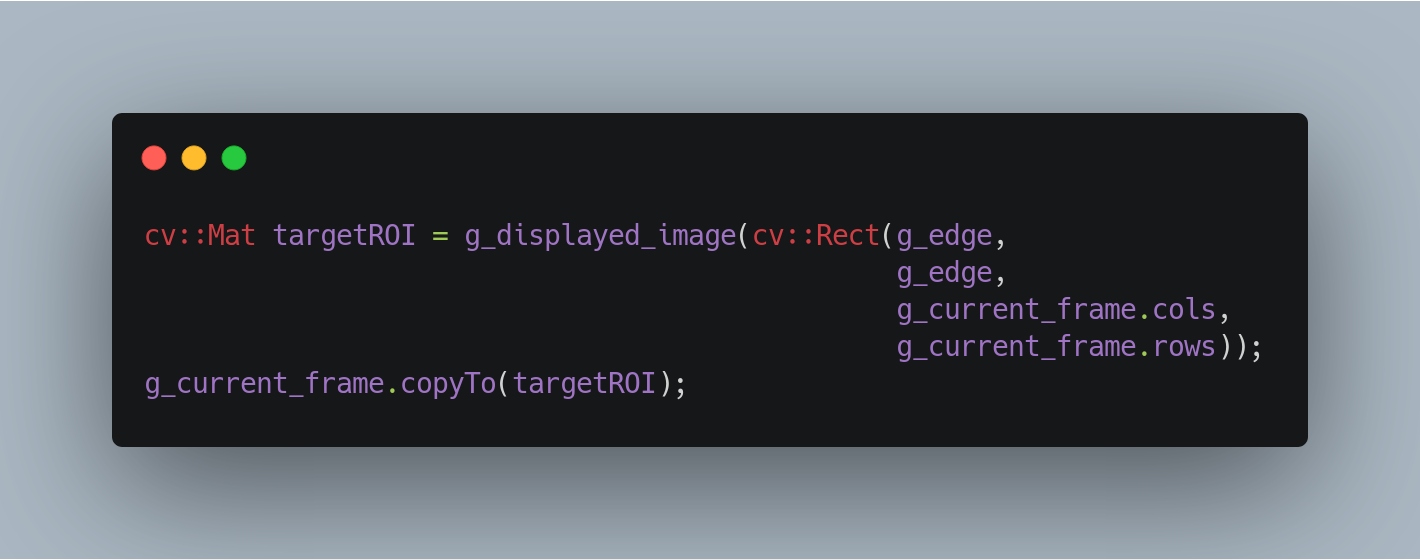
\includegraphics[width=\linewidth]{/home/fpvidal/Downloads/carbon(13)}


To perform the edge detection, we use the Canny filter:

% \begin{lstlisting}[language=c++]
% cv::Canny(blurred_frame, g_edge_frame, g_low_threshold, g_low_threshold * g_ratio, g_kernel_size);
% \end{lstlisting}
\begin{center}
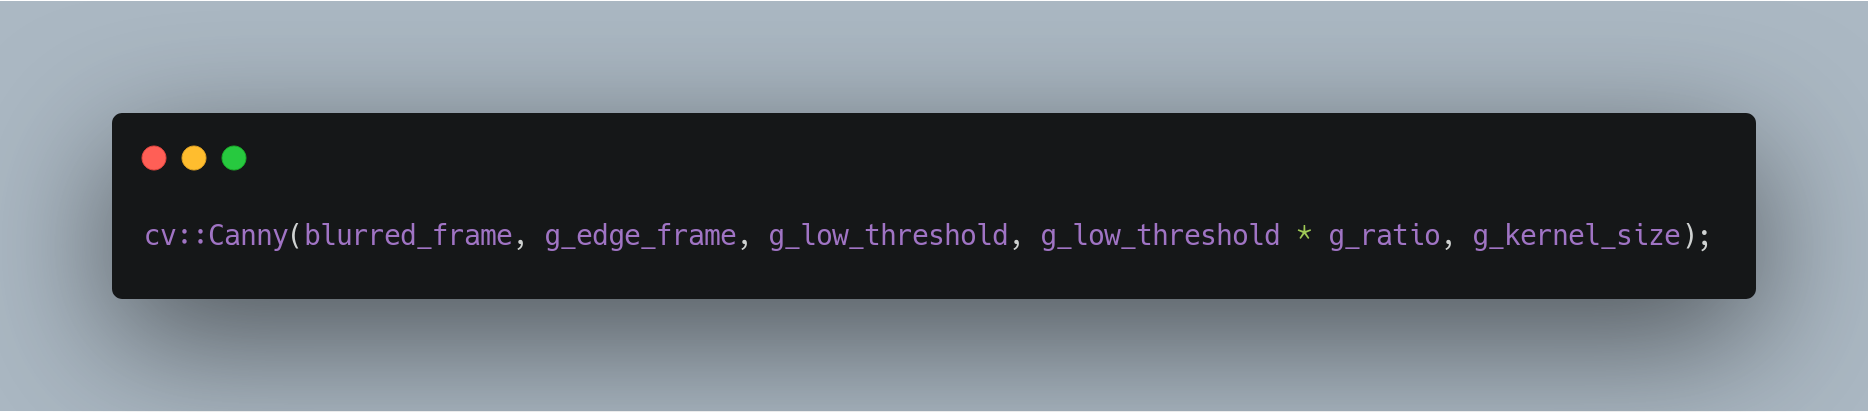
\includegraphics[width=\linewidth]{/home/fpvidal/Downloads/carbon(14)}
\end{center}

where the arguments are:
\begin{enumerate}
    \item \verb+blurred_frame+: Source image
    \item \verb+g_edge_frame+: Output of the detector
    \item \verb+g_low_threshold+: The value entered by the user moving the Trackbar
    \item \verb+g_low_threshold * g_ratio+: Set in the program as three times the lower threshold (following Canny's recommendation)
    \item \verb+g_kernel_size+: We defined it to be 3 (the size of the Sobel kernel to be used internally)
\end{enumerate}
For details about the Canny detector, you can check the lectures slides, last week's lab and the documentation from OpenCV (available at \url{https://docs.opencv.org/trunk/da/d5c/tutorial_canny_detector.html}).

Then convert the resulting image in RGB (see Lab~7 on \textit{Introduction to OpenCV}) and finally copy the result into the appropriate ROI:

% \begin{lstlisting}[language=c++]
% targetROI = g_displayed_image(cv::Rect(g_edge * 2 + g_current_frame.cols, g_edge, g_edge_frame.cols, g_edge_frame.rows));
%     g_edge_frame.copyTo(targetROI);
% \end{lstlisting}
\begin{center}
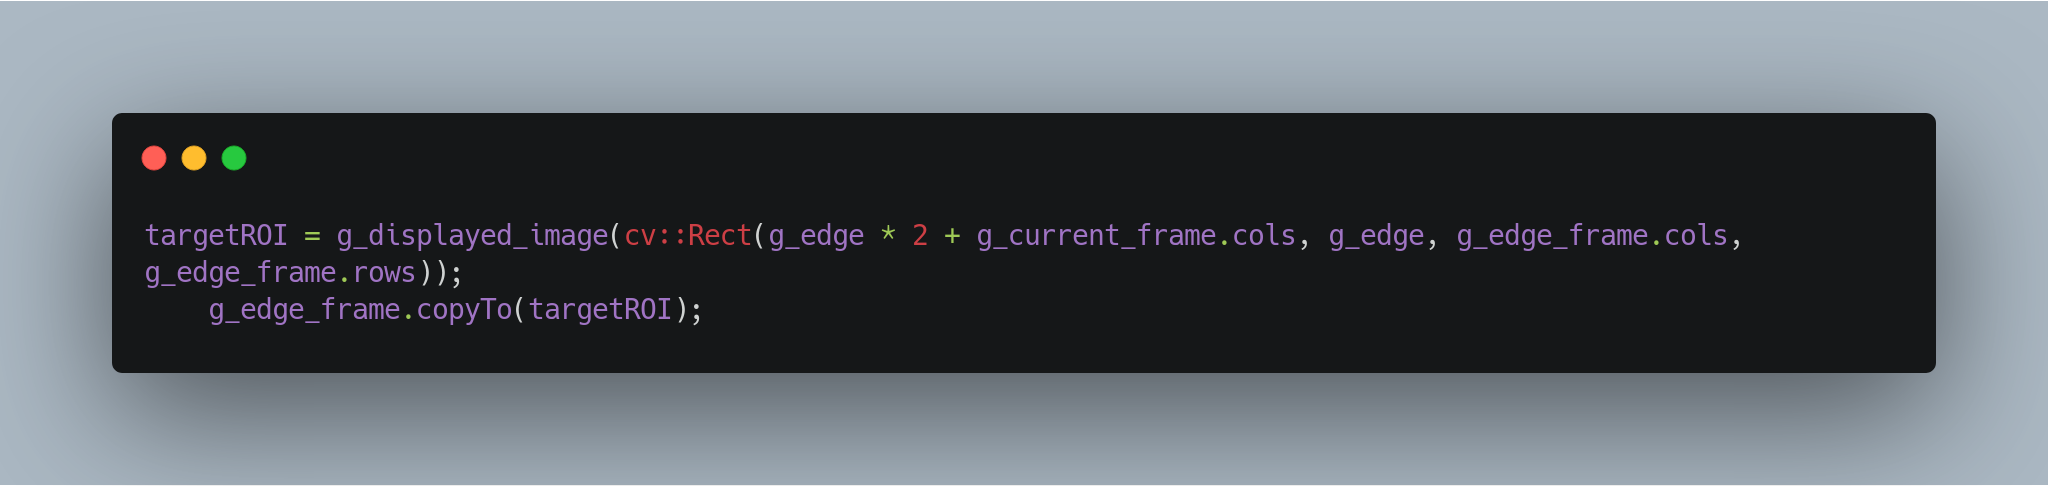
\includegraphics[width=\linewidth]{/home/fpvidal/Downloads/carbon(15)}
\end{center}

Finally, display \verb+g_displayed_image+ in the window (using \verb=cv::imshow=, see Labs~6 \&~7).




%%%%%%%%%%%%%%%%%%%%%%%%%%%%%%%%%%%%%%%%%%%%%%%%%%%%%%%%%%%%%%%%%%%%%%%%%%%%%%%%
\section{Video from a webcam}

Copy \verb+videoFromFile.cxx+ into \verb+videoFromCamera.cxx+. 
Make sure you update \verb+CMakeLists.txt+ so that \verb+videoFromCamera.cxx+ is compile, and linked against OpenCV's libraries.

The program takes two arguments from the command line:
\begin{itemize}
  \item A scaling factor to resize the input data (use 1 for no scaling);
  \item The output video file (optional).
\end{itemize}

% Use 
% \begin{lstlisting}[language=c++]
% 	// Open the video stream from the camera
% 	cv::VideoCapture video_capture(0);
% \end{lstlisting}
% instead of 
% \begin{lstlisting}[language=c++]
% 	// Open the video stream from a file
% 	cv::VideoCapture video_capture(input_file_name);
% \end{lstlisting}
\begin{center}
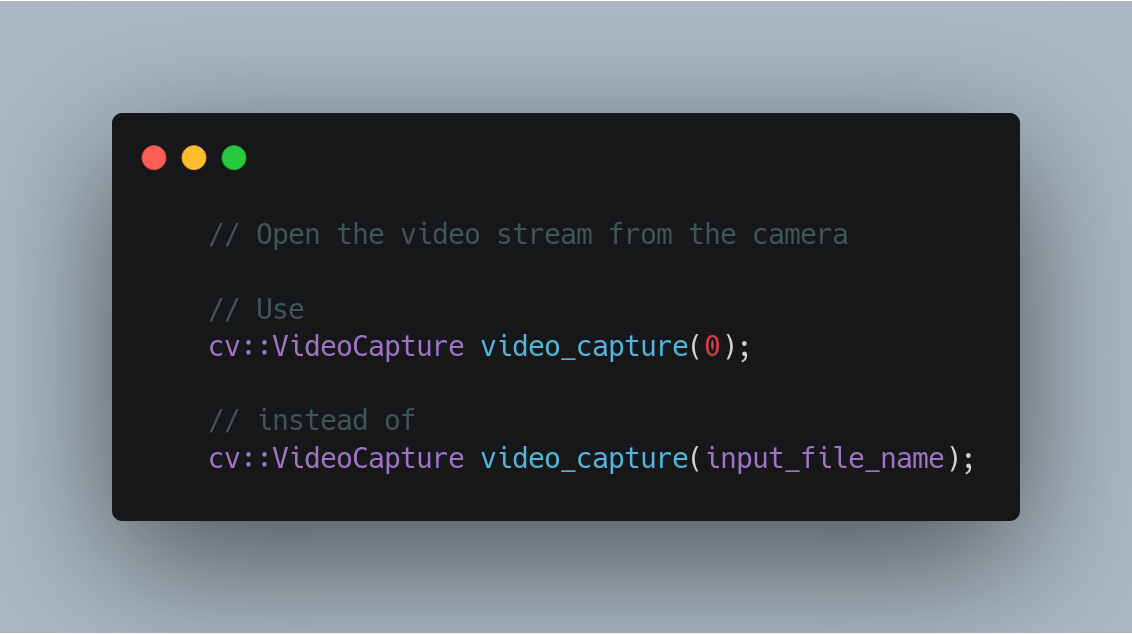
\includegraphics[width=0.8\linewidth]{/home/fpvidal/Downloads/carbon(16)}
\end{center}

Adapt the source code to take into account the changes in the command line arguments.
Also, set the number of frames per second to 15. 

Then you can create and process your own videos...
For example, Fig.~\ref{fig:screenshot2} shows my fish tank. You can also upload your video files on YouTube, see \url{https://www.youtube.com/watch?v=RbH2bdrNGbc} and \url{https://www.youtube.com/watch?v=RbH2bdrNGbc}.

 \begin{figure}[htbp]
  \centering
  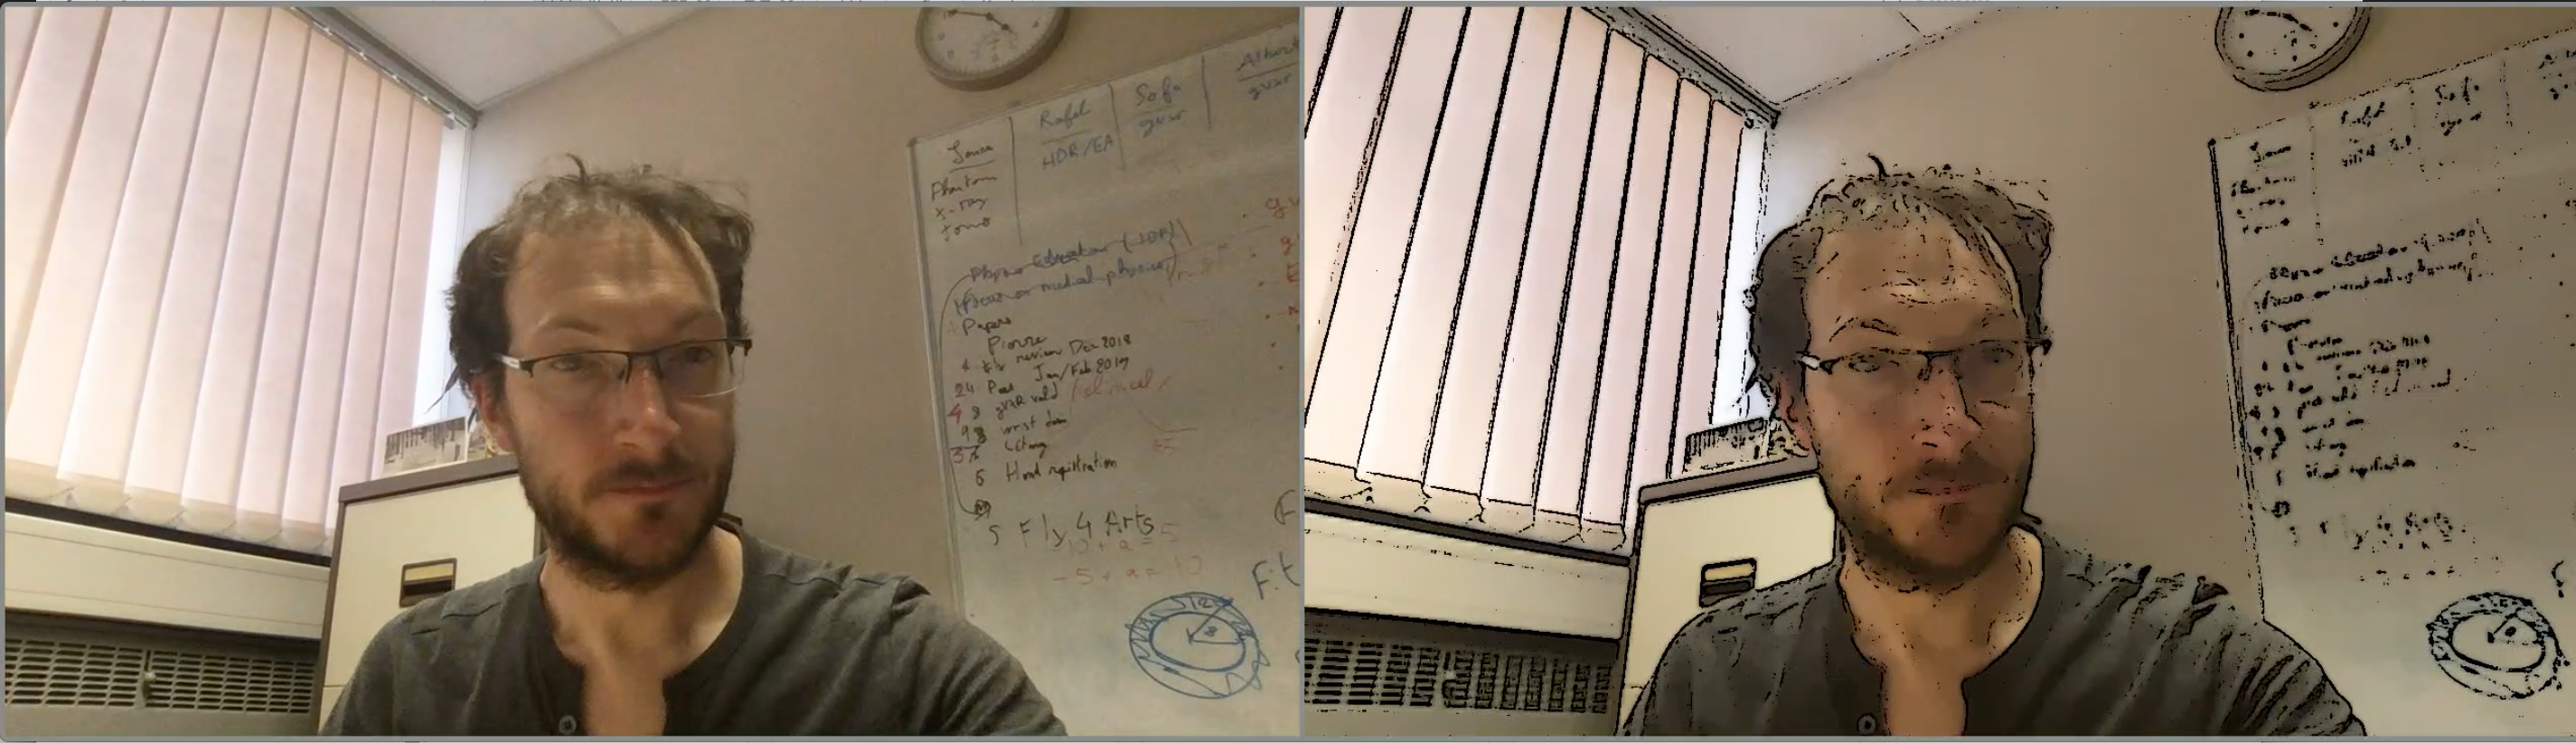
\includegraphics[width=\linewidth]{screenshot2}
  \caption{\label{fig:screenshot2}Screenshot.}
 \end{figure}



%\section{Gaussian Pyramid}
%
%If you are done, investigate the use of Gaussian pyramids and try the code provided at 
% \url{http://docs.opencv.org/2.4/doc/tutorials/imgproc/pyramids/pyramids.html}. 



%%%%%%%%%%%%%%%%%%%%%%%%%%%%%%%%%%%%%%%%%%%%%%%%%%%%%%%%%%%%%%%%%%%%%%%%%%%%%%%%
\end{document}
